\documentclass[10pt]{beamer}

\usetheme{metropolis}
\usepackage{appendixnumberbeamer}

\usepackage{booktabs}
\usepackage[scale=2]{ccicons}
\usepackage{graphicx}
\usepackage{hyperref}
\usepackage{circuitikz}
\usepackage{pdflscape}
\usepackage{smartdiagram}

\usepackage{color}
\usepackage{listings}

\lstset{
	basicstyle=\footnotesize\ttfamily,
    keepspaces=true,
    showstringspaces=false,
    language=PHP,
    commentstyle=\ttfamily,
}

\usepackage[OT4]{polski}
\usepackage[utf8]{inputenc}

\usepackage{pgfplots}
\usepgfplotslibrary{dateplot}

\usepackage{xspace}
\newcommand{\themename}{\textbf{\textsc{metropolis}}\xspace}

\setbeamertemplate{frame footer}{}
\setbeamertemplate{frame numbering}{}

\usetikzlibrary{shapes,arrows}

\tikzstyle{decision} = [diamond, draw, fill=blue!20, 
    text width=4.5em, text badly centered, node distance=3cm, inner sep=0pt]
\tikzstyle{block} = [rectangle, draw, fill=blue!20, 
    text width=5em, text centered, rounded corners, minimum height=4em]
\tikzstyle{line} = [draw, -latex']
\tikzstyle{cloud} = [draw, ellipse,fill=red!20, node distance=3cm,
    minimum height=2em]


\title{KISS, DRY, YAGNI i inne}

\subtitle{Projektowanie i programowanie systemów internetowych I}
\author{mgr inż. Krzysztof Rewak}
\date{\today}
\institute{Wydział Nauk Technicznych i Ekonomicznych \\ Państwowa Wyższa Szkoła Zawodowa im. Witelona w Legnicy}

\begin{document}

\maketitle

\begin{frame}{Plan prezentacji}
  \setbeamertemplate{section in toc}[sections numbered]
  \tableofcontents[hideallsubsections]
\end{frame}


\begin{frame}{Dobre praktyki programistyczne}
	Czym są dobre praktyki programistyczne?
\end{frame}

\begin{frame}{Dobre praktyki programistyczne}
	Najprawdopodobniej każdy programista może przedstawić własny zestaw praktyk, które uważa za dobre.
\end{frame}

\begin{frame}{Dobre praktyki programistyczne}
	(ciekawą rzeczą oczywiście będzie porównanie dwóch takich zestawów i przekonanie się, że część \emph{zasad} brzmi podobnie, część dotyczy całkowicie różnych rzeczy, a część w zasadzie sobie przeczy)
\end{frame}

\begin{frame}{Dobre praktyki programistyczne}
	Podobnie jak z zasadami SOLID, pewne rzeczy bardzo często są odkrywane przez programistów \emph{samodzielnie}. Dobrze jednak znać najpopularniejsze reguły, aby umieć odnaleźć się w prawdziwym świecie.
\end{frame}

\section{KISS}

\begin{frame}{KISS}
	\textbf{KISS}.
	
	\emph{Keep It Simple, Stupid}.
	
	\emph{Nie komplikuj, głupcze}.
\end{frame}

\begin{frame}{KISS}
	Apoteoza minimalizmu, implementacja brzytwy Ockhama, leonardowska \emph{Prostota jest szczytem wyrafinowania}.
\end{frame}

\begin{frame}{KISS}
	KISS jest ciekawym zagadnieniem, ponieważ stosowane jest w wielu dziedzinach: od projektowania silników odrzutowców począwszy, a na tworzeniu filmów animowanych skończywszy.
\end{frame}

\begin{frame}{KISS}
	Czym KISS będzie w programowaniu? 
\end{frame}

\begin{frame}{KISS}
	Warto wspomnieć przynajmniej dwa podejścia: upraszczanie nazewnictwa raz upraszczanie logiki biznesowej.
\end{frame}

\begin{frame}{KISS w nazewnictwie}
	Wyobraźmy sobie projekt, w którym ktoś nagorliwie nazywa... wszystko.
\end{frame}

\begin{frame}
	\begin{figure} \centering
		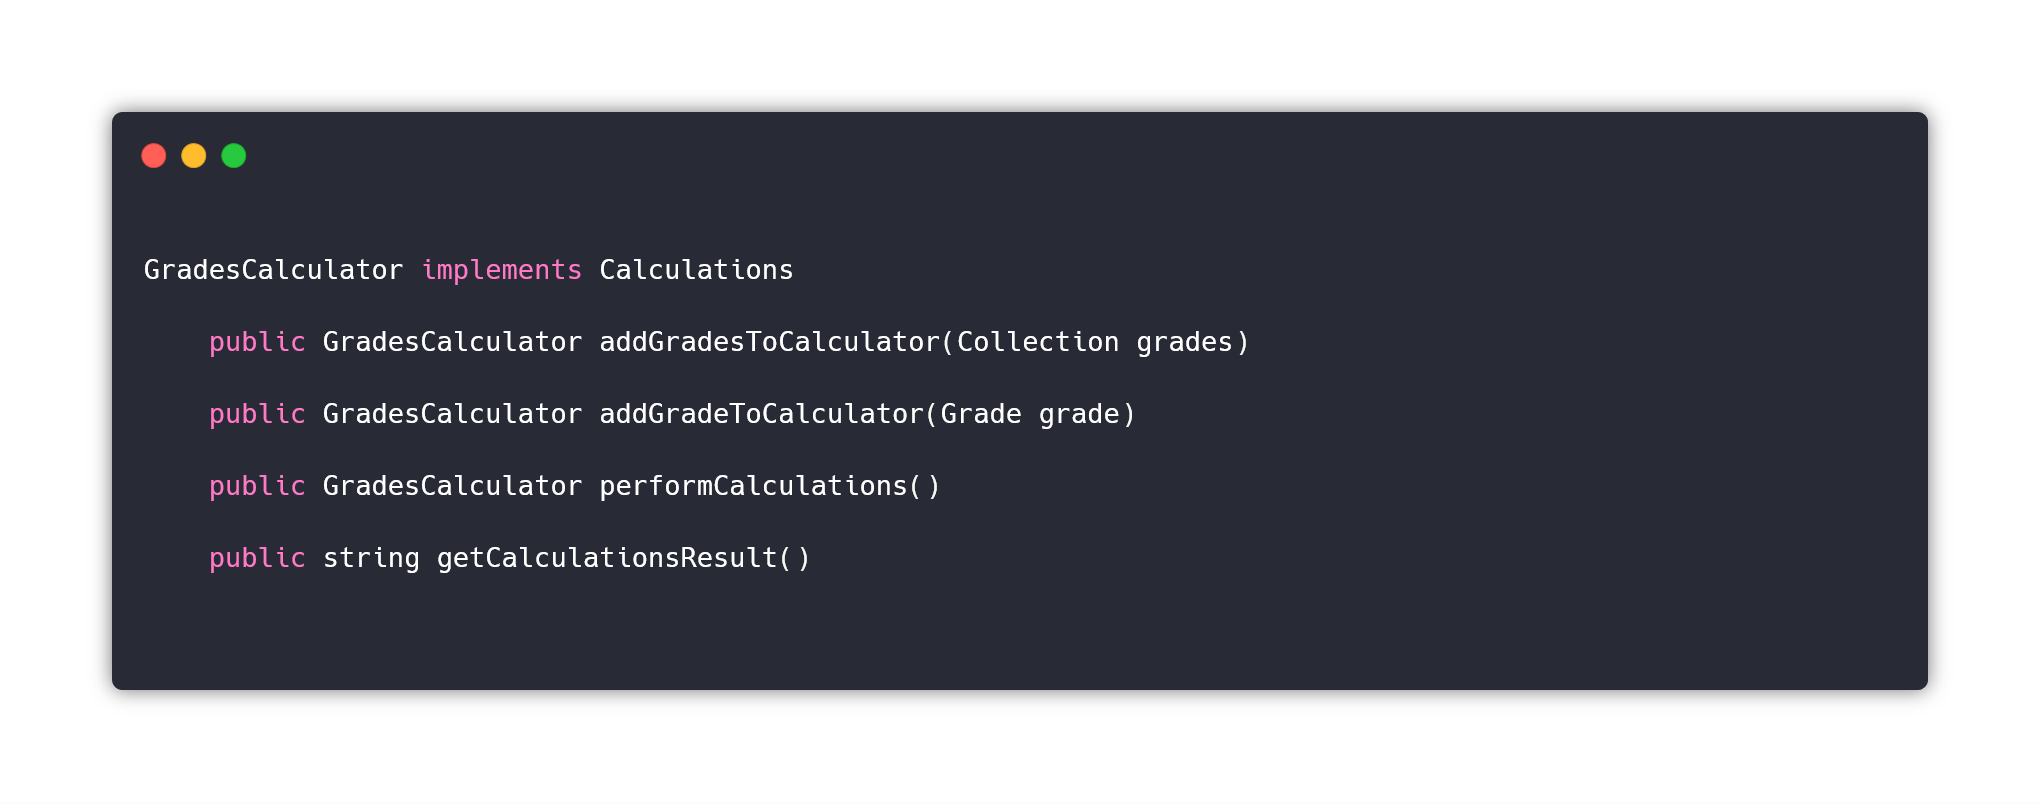
\includegraphics[width=\textwidth]{kiss00.png}
	\end{figure}
\end{frame}

\begin{frame}{KISS w nazewnictwie}
	Czy naprawdę sens ma podkreślanie, że dodajemy oceny do kalkulatora w nazwie metody? 
\end{frame}

\begin{frame}
	\begin{figure} \centering
		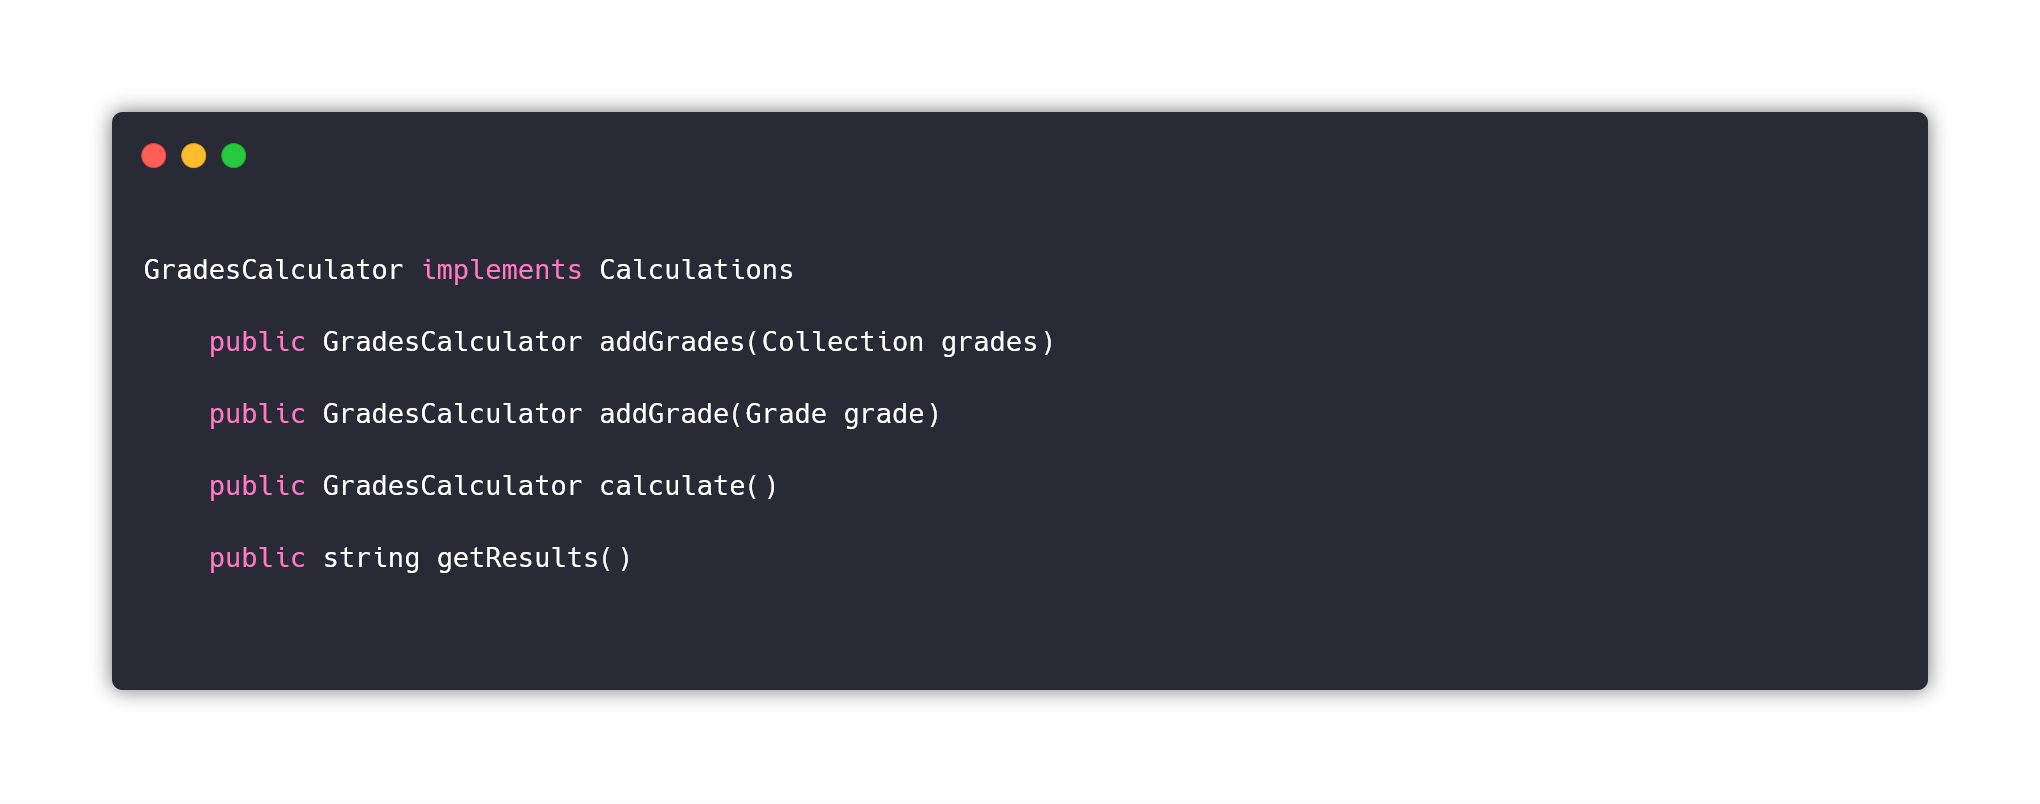
\includegraphics[width=\textwidth]{kiss01.png}
	\end{figure}
\end{frame}

\begin{frame}{KISS w logice biznesowej}
	Lepiej? Pewnie, że lepiej.
	
	Ale spójrzmy na to jak działa taki kalkulator.
\end{frame}

\begin{frame}
	\begin{figure} \centering
		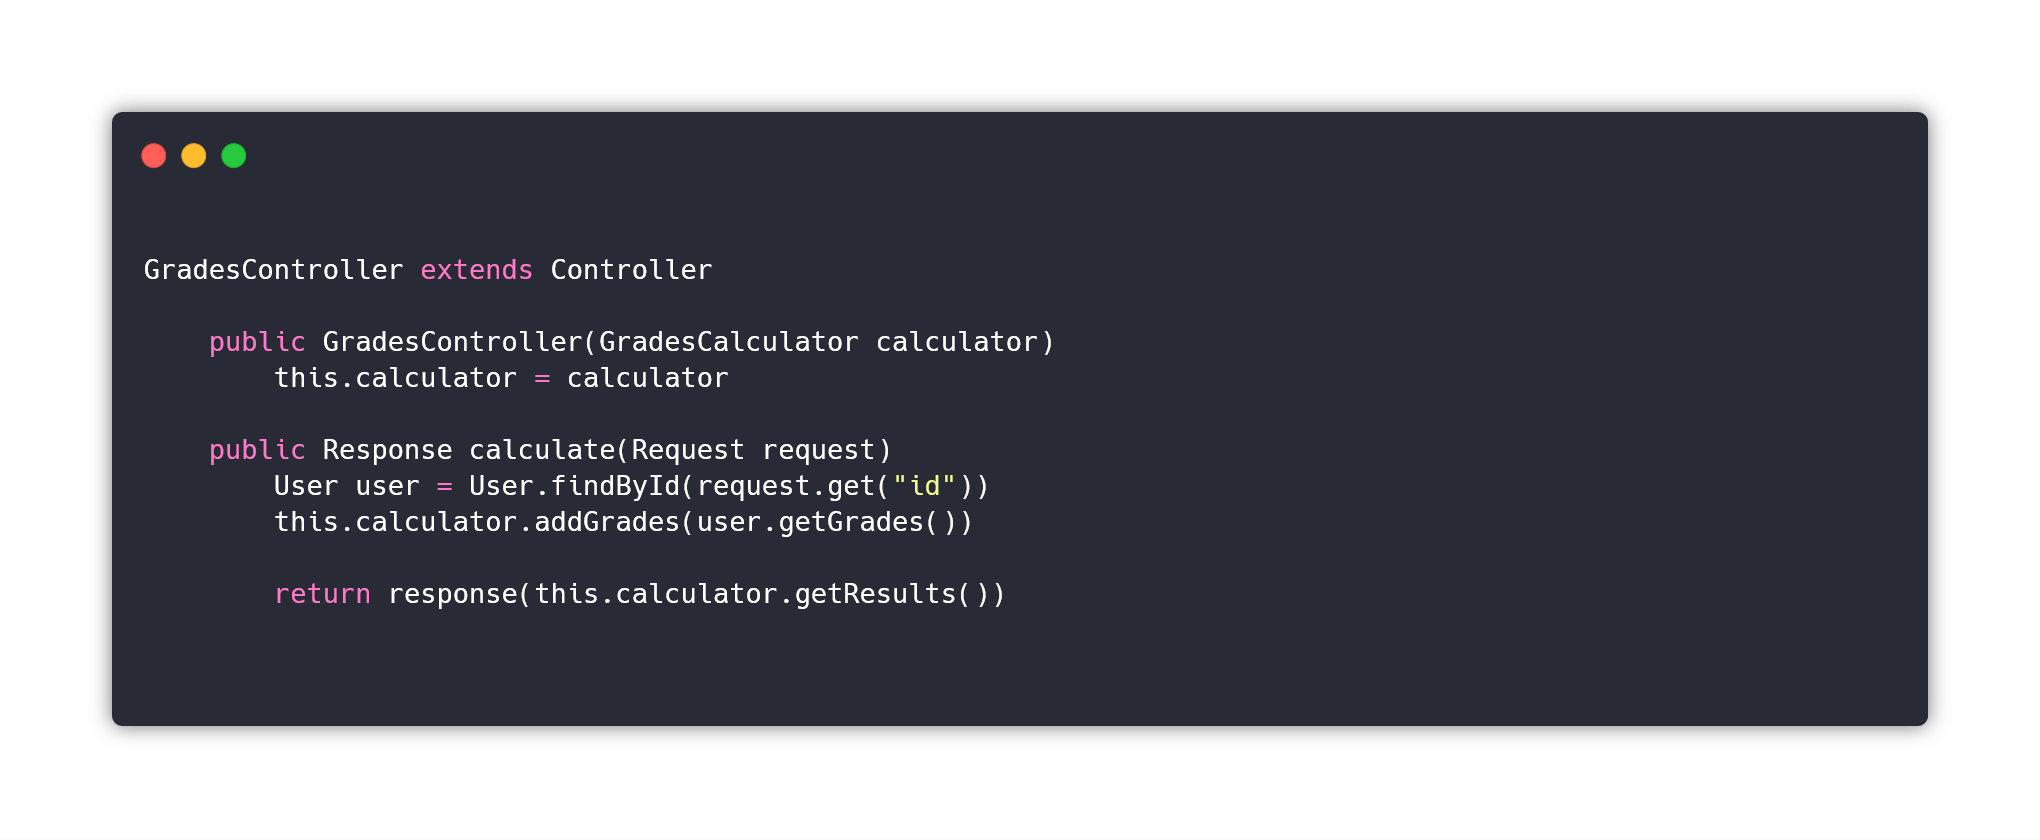
\includegraphics[width=\textwidth]{kiss02.png}
	\end{figure}
\end{frame}

\begin{frame}{KISS w logice biznesowej}
	Kod powyżej się nie uruchomi, ponieważ nakomplikowaliśmy z interfejsem kalkulatora.
\end{frame}

\begin{frame}
	\begin{figure} \centering
		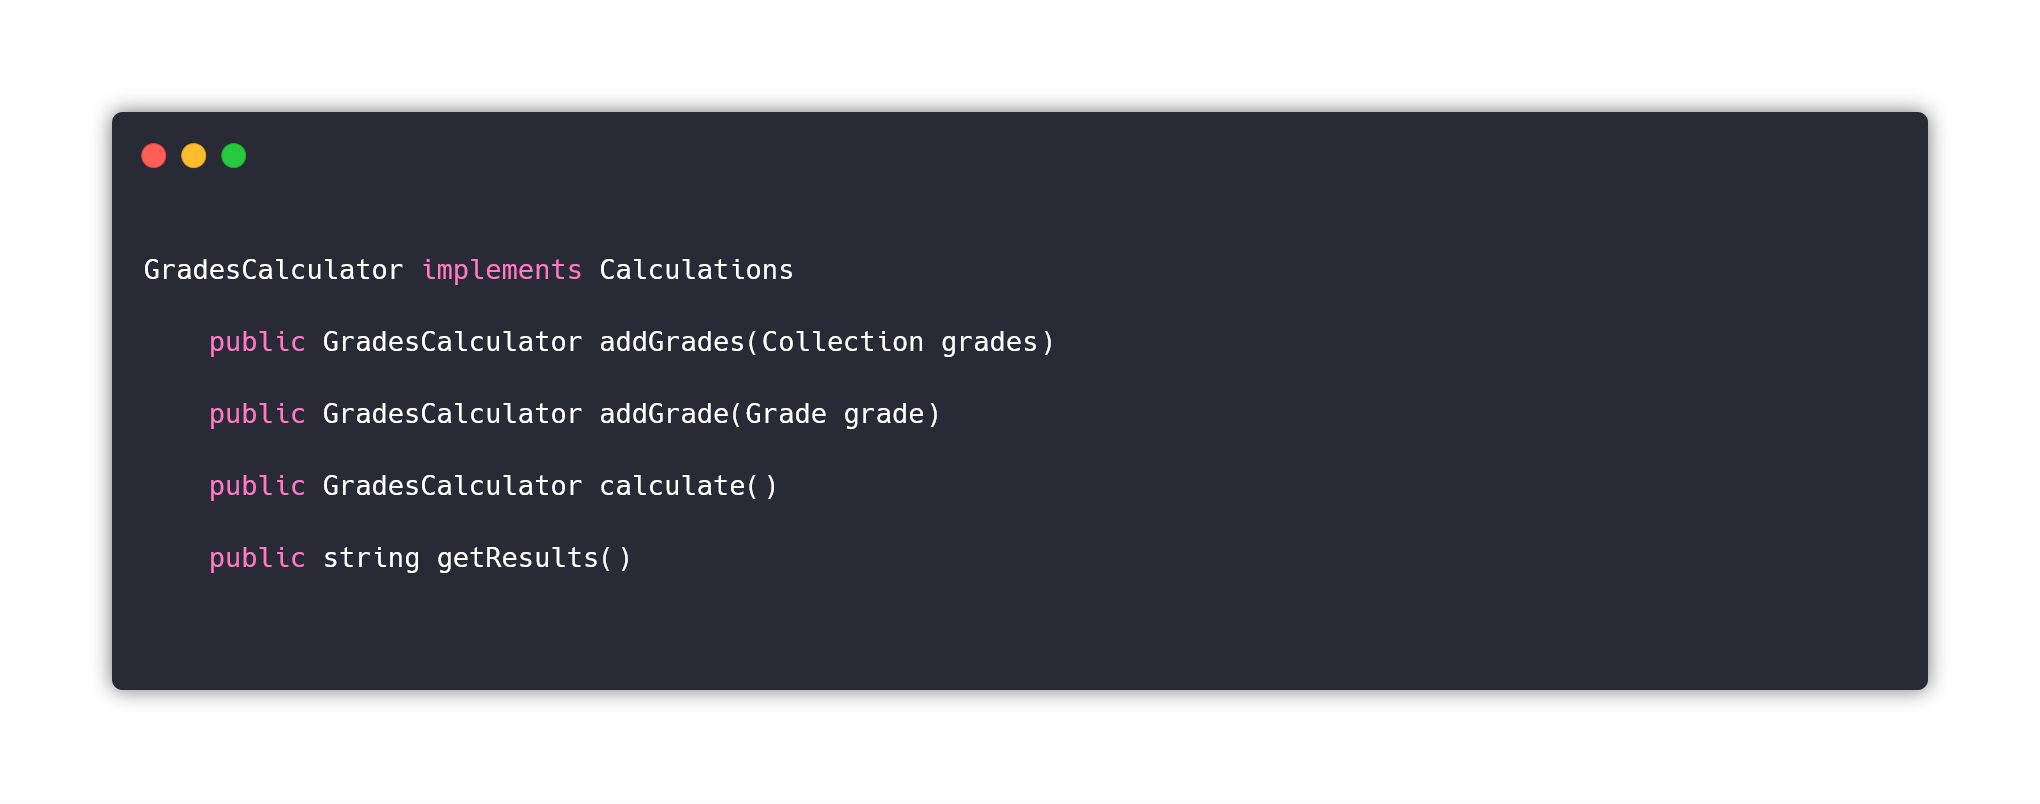
\includegraphics[width=\textwidth]{kiss01.png}
	\end{figure}
\end{frame}

\begin{frame}{KISS w logice biznesowej}
	Jako autorzy tego kalkulatora doskonale wiemy, że nie ma co brać wyniku jeżeli uprzednio nie uruchomimy obliczania tegoż wyniku. To logiczne!
	
	Problem polega na tym, że dla innego programisty nie będzie to wcale takie proste. Pamiętać, że musimy wywołać jakąś metodę zanim wywołamy inną? \emph{Keep it simple, stupid!}
\end{frame}

\begin{frame}{KISS w logice biznesowej}
	Jakie rozwiązanie powinno nam przyjść do głowy, aby uprościć taki kalkulator?
	
	Dodać rzucanie wyjątku w momencie, gdy ktoś uruchomi pobranie wyniku? Czy to będzie faktycznie prostsze?
\end{frame}

\begin{frame}{KISS w logice biznesowej}
	A może zahermetyzować obliczenia i wywołać je przy pobieraniu wyniku? Ale co z SRP?
\end{frame}

\begin{frame}{KISS w logice biznesowej}
	Im większa klasa, tym więcej rzeczy będzie można prawdopodobnie uprościć. Spójrzmy na kontroler w serwisie randkowym, który umożliwia nadpisanie danych o użytkowniku:
\end{frame}

\begin{frame}
	\begin{figure} \centering
		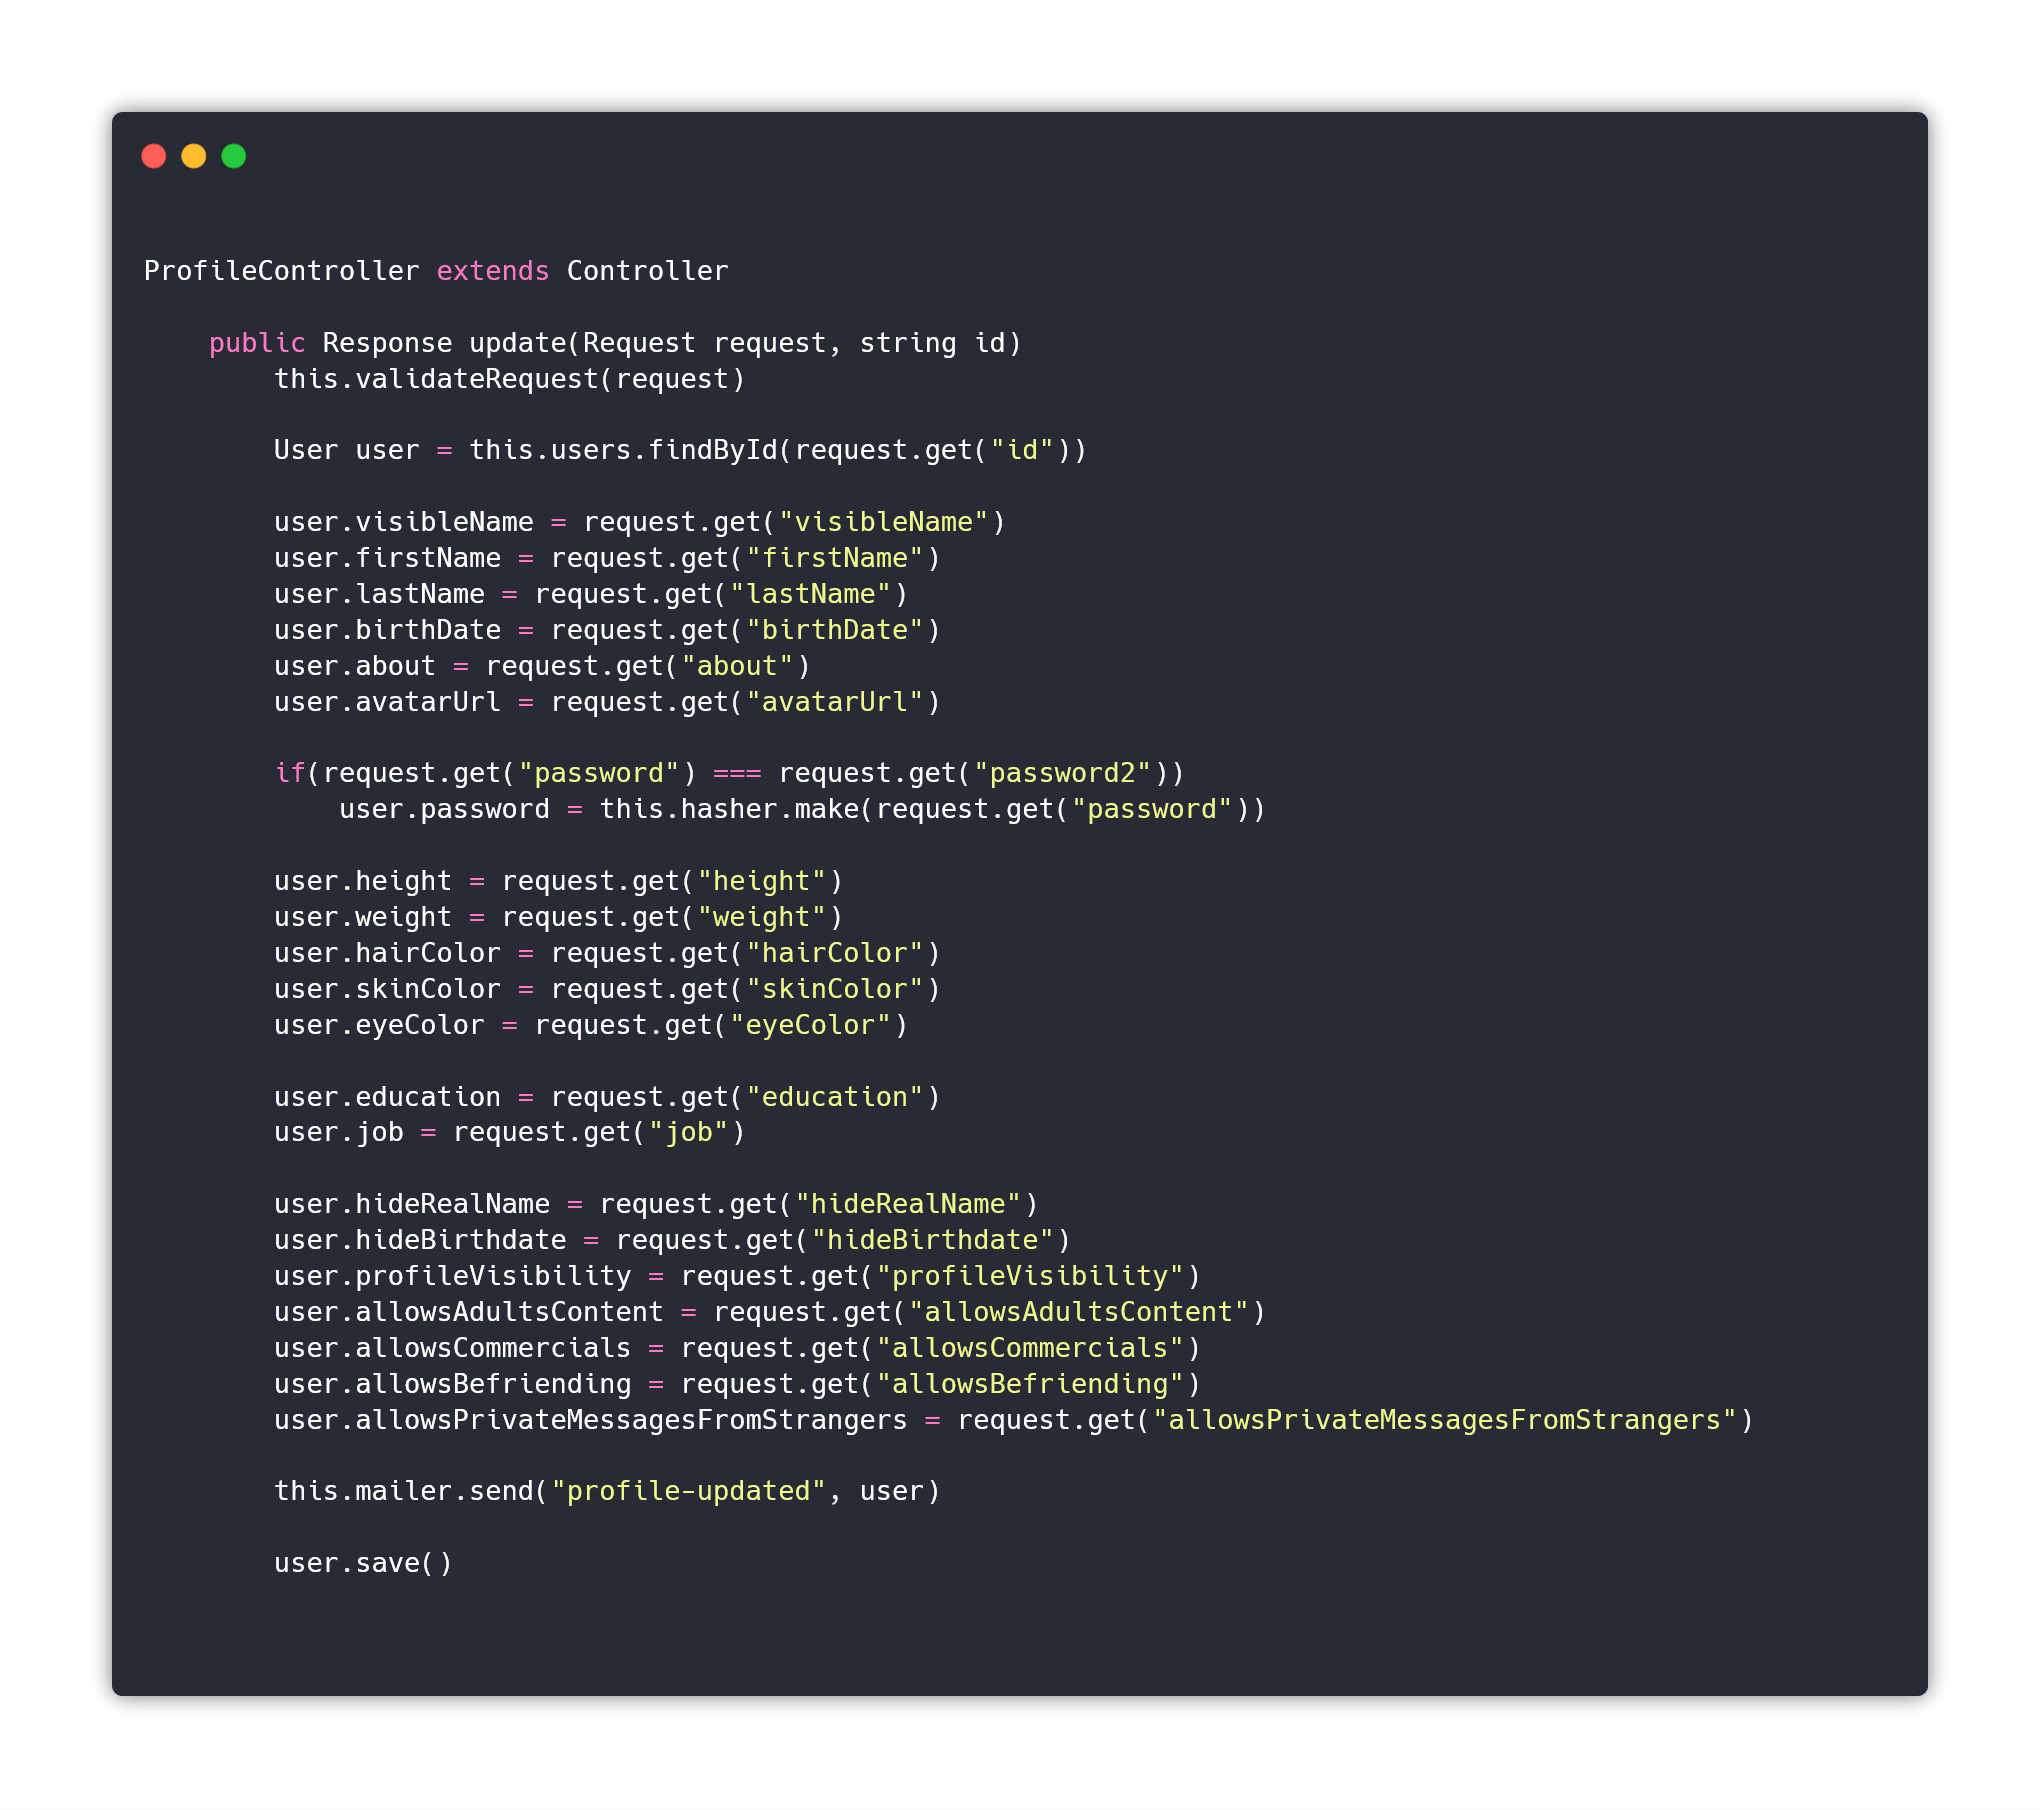
\includegraphics[width=\textwidth]{kiss03.png}
	\end{figure}
\end{frame}

\begin{frame}{KISS}
	Im większa klasa, tym więcej rzeczy faktycznie można uprościć.
	
	Im prostszy kod, tym łatwiej się go czyta. Może warto zastanowić się czy programista więcej kodu w swoim życiu przeczyta, czy wyprodukuje?
\end{frame}

\section{DRY}

\begin{frame}{DRY}
	\textbf{DRY}.
	
	\emph{Don't repeat yourself}.
	
	\emph{Nie powtarzaj się}.
\end{frame}

\begin{frame}{DRY}	
	\emph{Every piece of knowledge must have a single, unambiguous, authoritative representation within a system}.
	
	\emph{Każdy fragment domeny musi mieć jedną, jednoznaczną i wyraźną reprezentację w systemie.}
	
	-- \emph{The Pragmatic Programmer}, Andy Hunt i Dave Thomas
\end{frame}

\begin{frame}{DRY}
	DRY, według jego autorów, dotyczy przede wszystkim kodu, ale również baz danych, testów, wdrażania, a nawet dokumentacji.
\end{frame}

\begin{frame}{DRY}
	Do podstawowego zastosowania młodzi programiści dochodzą bardzo szybko. Bo czymże innym jest zamykanie pewnych obszarów kodu do funkcji, jeżeli nie wykrozystaniem metodologii DRY?
\end{frame}

\begin{frame}
	\begin{figure} \centering
		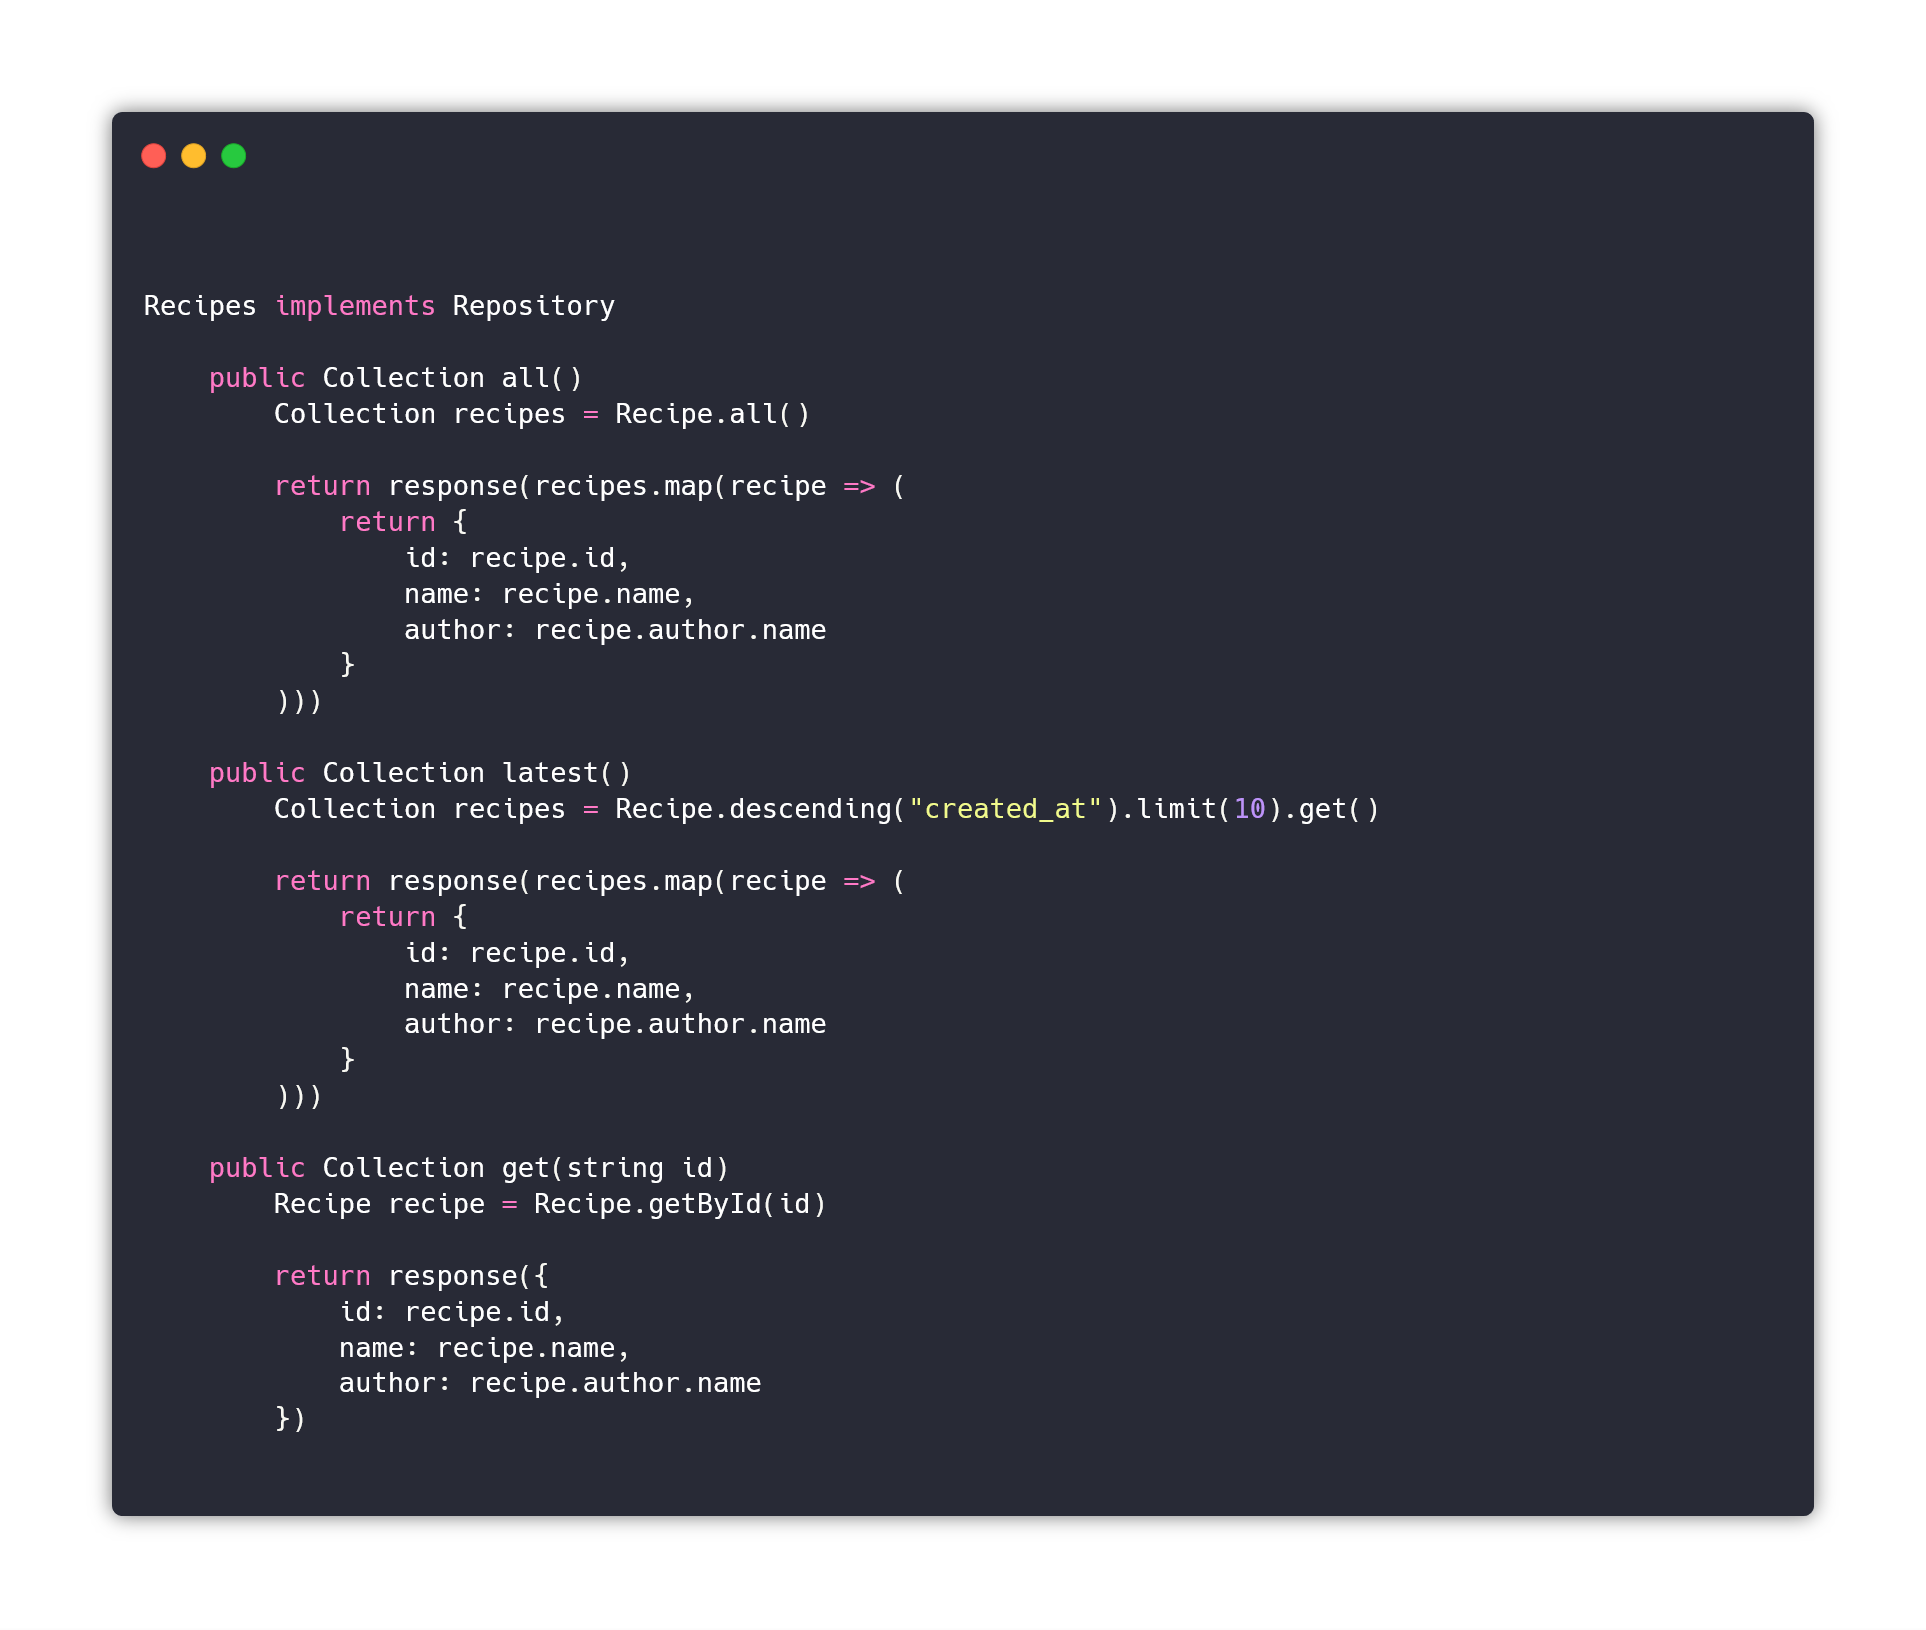
\includegraphics[width=\textwidth]{dry00.png}
	\end{figure}
\end{frame}

\begin{frame}
	\begin{figure} \centering
		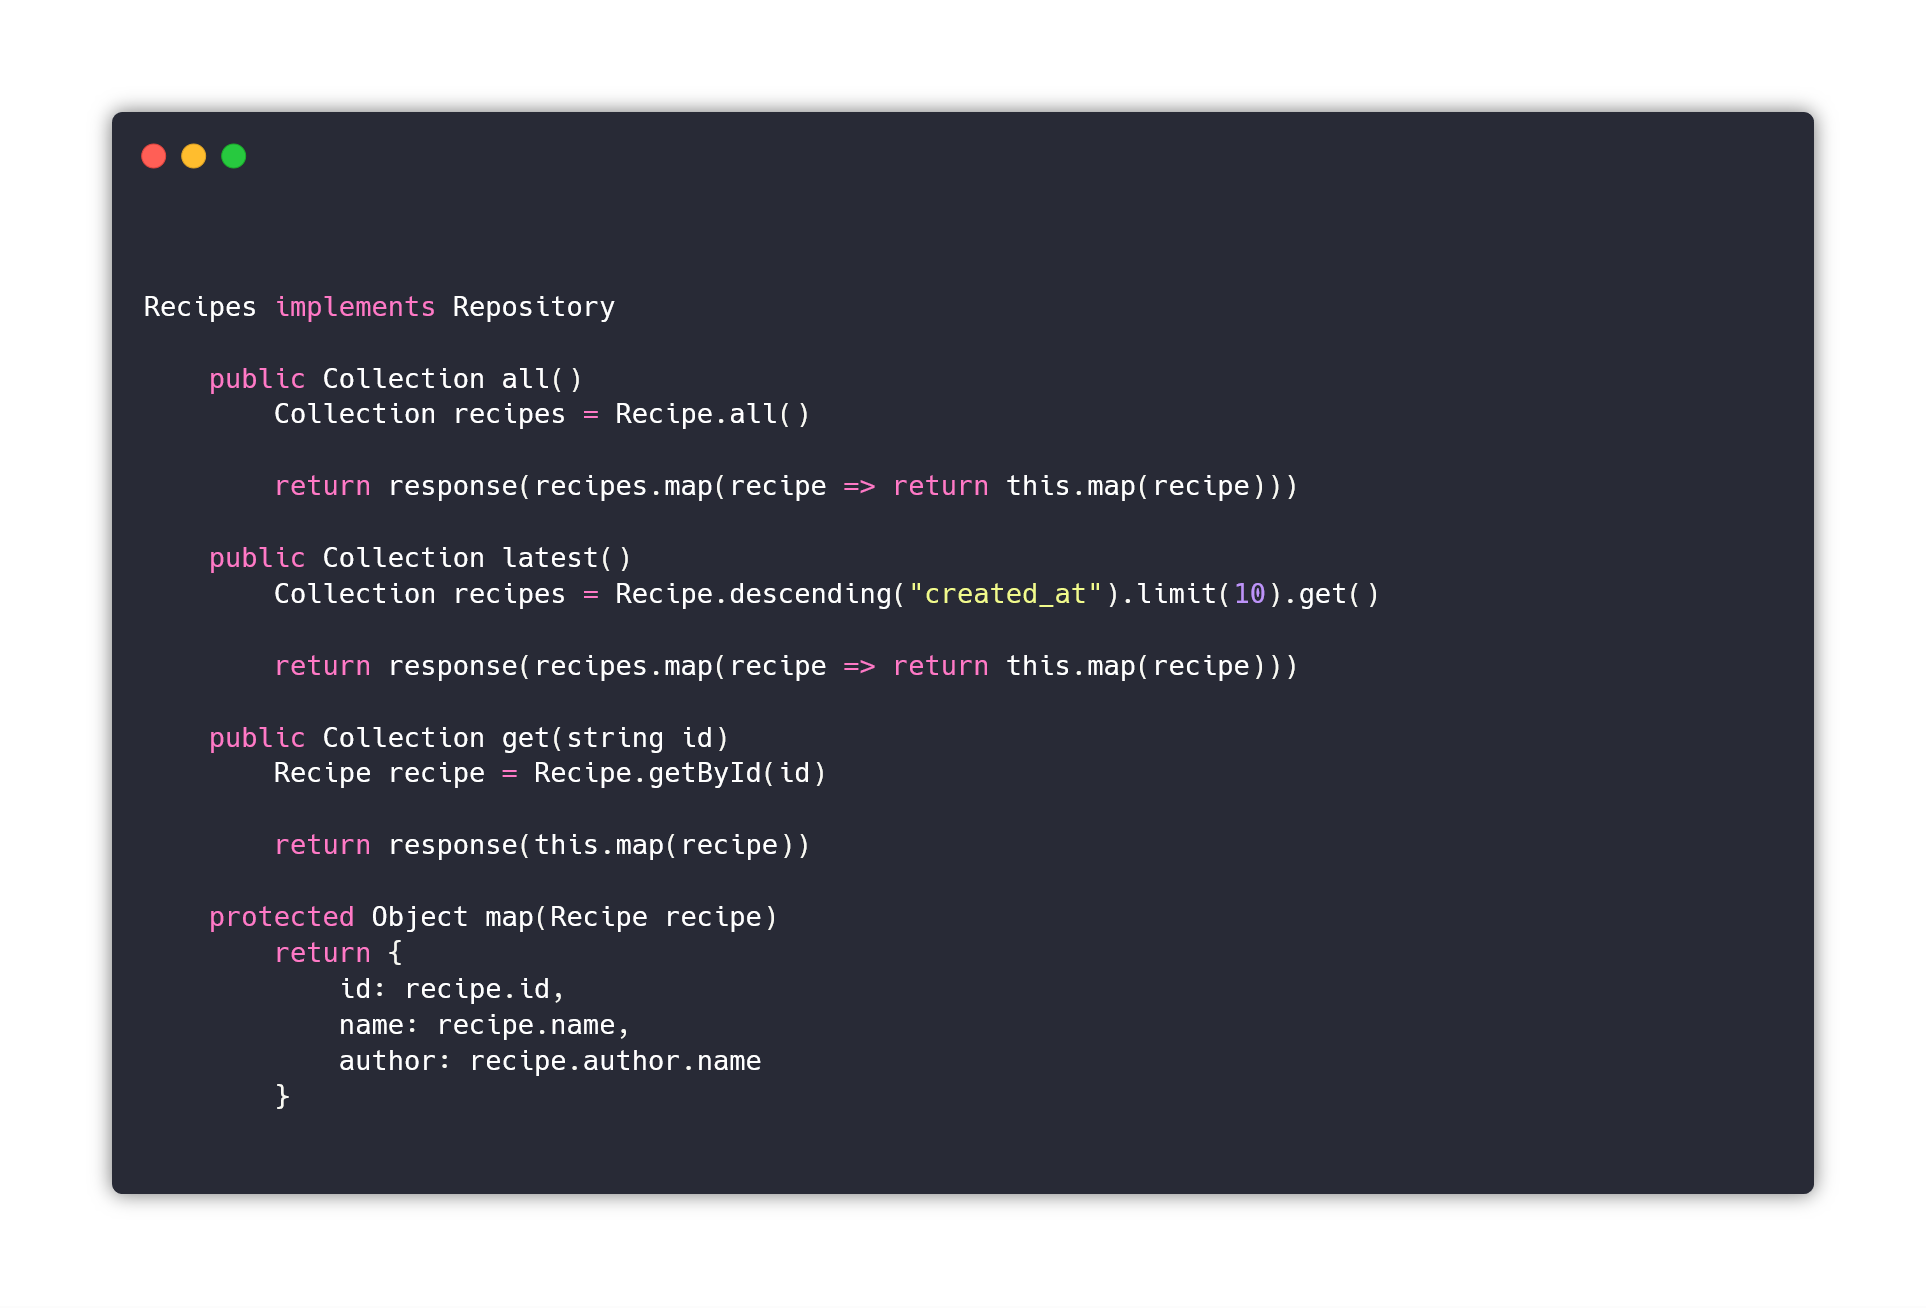
\includegraphics[width=\textwidth]{dry01.png}
	\end{figure}
\end{frame}

\begin{frame}{DRY}
	Nie tylko wydzielanie funkcji i metod pomaga w stosowaniu DRY.
\end{frame}

\begin{frame}
	\begin{figure} \centering
		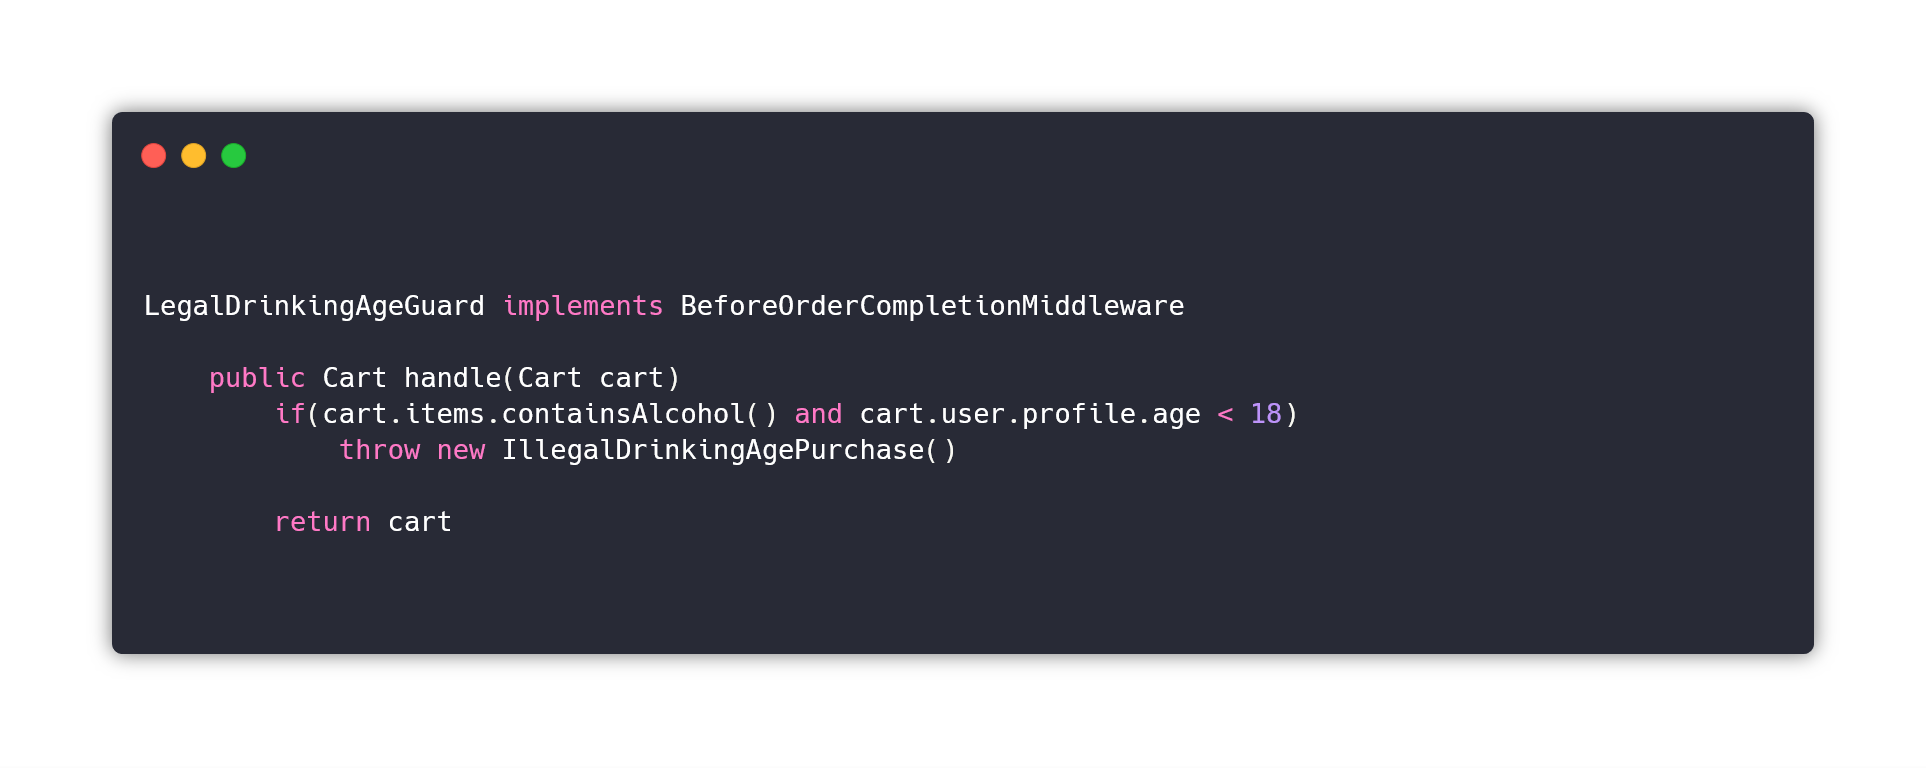
\includegraphics[width=\textwidth]{dry02.png}
	\end{figure}
\end{frame}

\begin{frame}{DRY}
	Bardzo dobrą praktyką jest korzystanie z nazwanych stałych, aby nie powtarzać wielokrotnie tych samych \emph{magicznych liczb}.
\end{frame}

\begin{frame}
	\begin{figure} \centering
		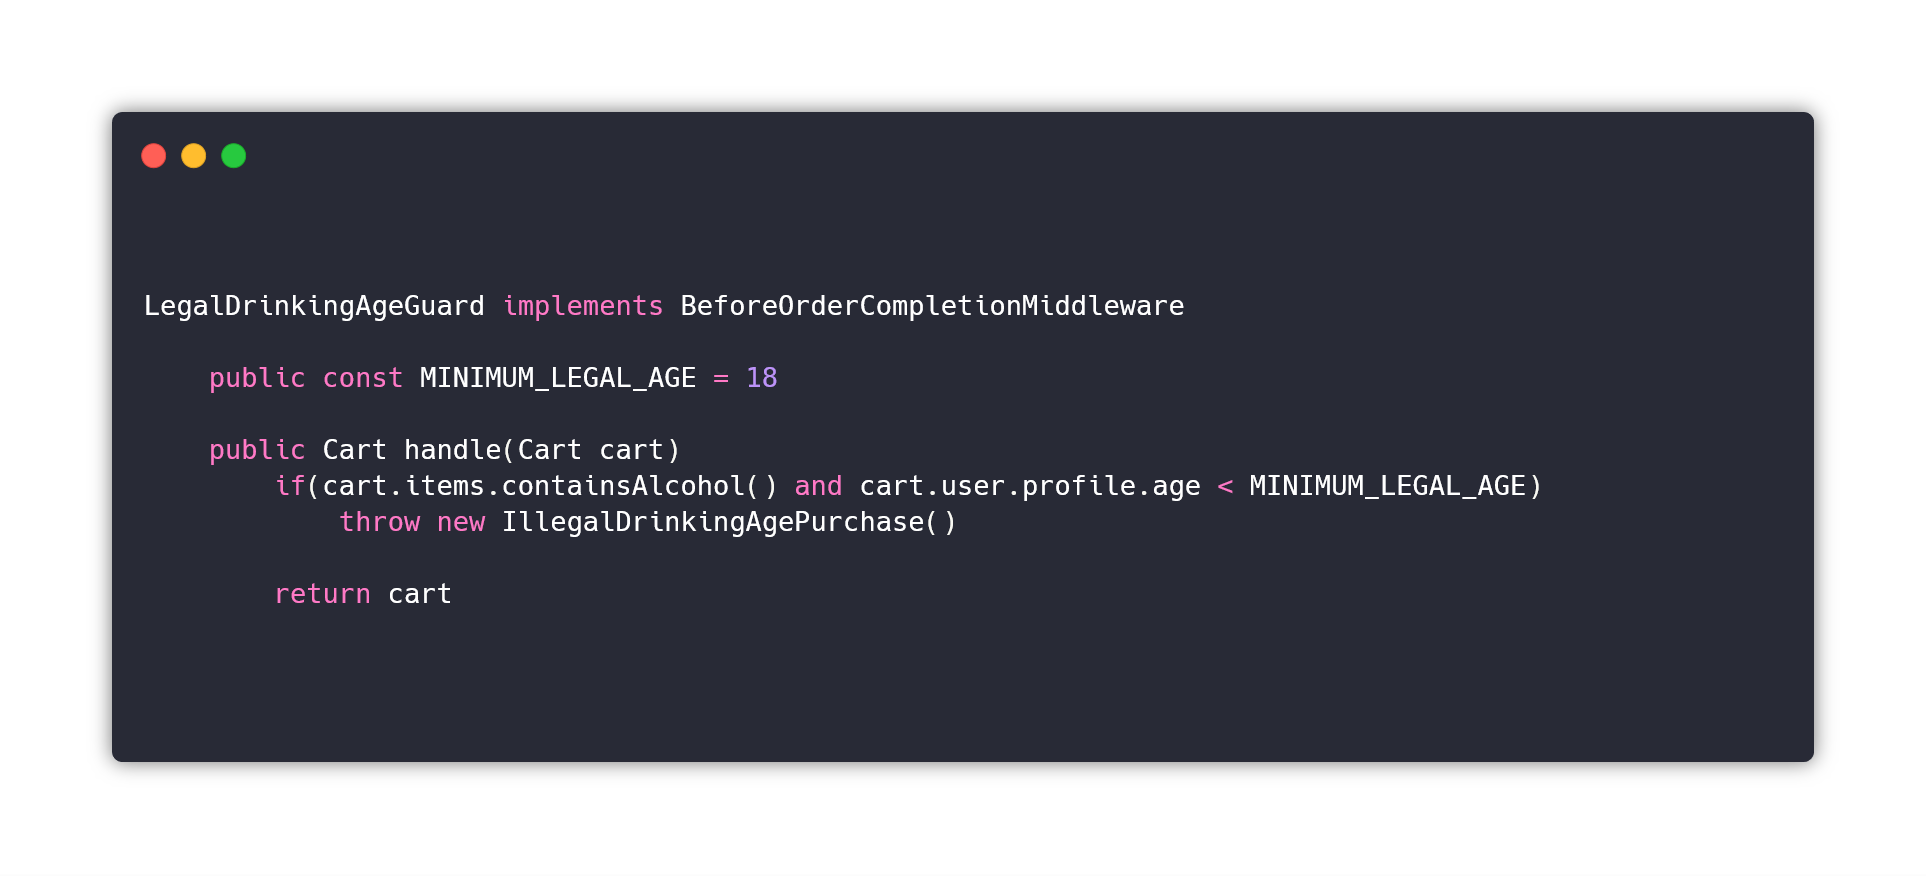
\includegraphics[width=\textwidth]{dry03.png}
	\end{figure}
\end{frame}

\begin{frame}{DRY}
	DRY należy rozumieć nie tylko na poziomie metod w klasach, ale również jako regułę dla całych projektów.
\end{frame}

\begin{frame}{DRY}
	Czy pisanie za każdym razem od nowa tych samych funkcjonalności ma sens? W kończy powtarzamy kolejny i kolejny raz tą samą rejestrację użytkownika, ten sam mechanizm wysyłania mejla z potwierdzeniem, to samo wylogowanie, to samo uwierzytelnienie JWT, ten sam system praw...
\end{frame}

\begin{frame}{DRY}
	Zatem czy używanie frameworka wpisuje się w regułę DRY?
\end{frame}

\begin{frame}{DRY}
	A może wewnątrz frameworka warto stworzyć własny zestaw do postawienia świeżego projektu? Albo własny szkielet pod kolejnego CRUD-a? Albo własną implementację systemu kolejkowego?
\end{frame}

\begin{frame}{DRY}
	Grunt to to, aby \emph{nie powtarzać} swojej pracy.
	
	I nie dlatego, że ktoś napisał o tym w swojej książce, ale przede wszystkim dlatego, że każda rzeczy powtórzona $n$ razy, za którymś razem zostanie powtórzona błędnie.
\end{frame}

\section{YAGNI}

\begin{frame}{YAGNI}
	\textbf{YAGNI}.
	
	\emph{You aren't gonna need it}.
	
	\emph{Nie będziesz tego potrzebować}.
\end{frame}

\begin{frame}{YAGNI}
	Dwie przedstawione wcześniej reguły (podobnie jak zeszłowykładowy SOLID) mówią, że warto zastanowić się nad upraszczaniem kodu lub budową pewnej abstrakcji, aby łatwiej nam się żyło w przyszłości.
\end{frame}

\begin{frame}{YAGNI}
	YAGNI na pierwszy rzut zaleca coś całkowicie innego.
	
	Dopóty programista nie powinien dodawać żadnych funkcjonalności, dopóki nie będą one naprawde potrzebne.
\end{frame}

\begin{frame}{YAGNI}
	\emph{Always implement things when you actually need them, never when you just foresee that you need them.}
	
	\emph{Zawsze programuj rzeczy, kiedy faktycznie ich potrzebujesz. Nigdy, kiedy po prostu przewidujesz, że będziesz ich potrzebować.}
	
	-- Ron Jeffries 
\end{frame}

\begin{frame}{YAGNI}
	Prostym przykładem może byc otrzymanie od klienta zadania utworzenia endpointa do uwierzytelniania użytkowników.
\end{frame}

\begin{frame}
	\begin{figure} \centering
		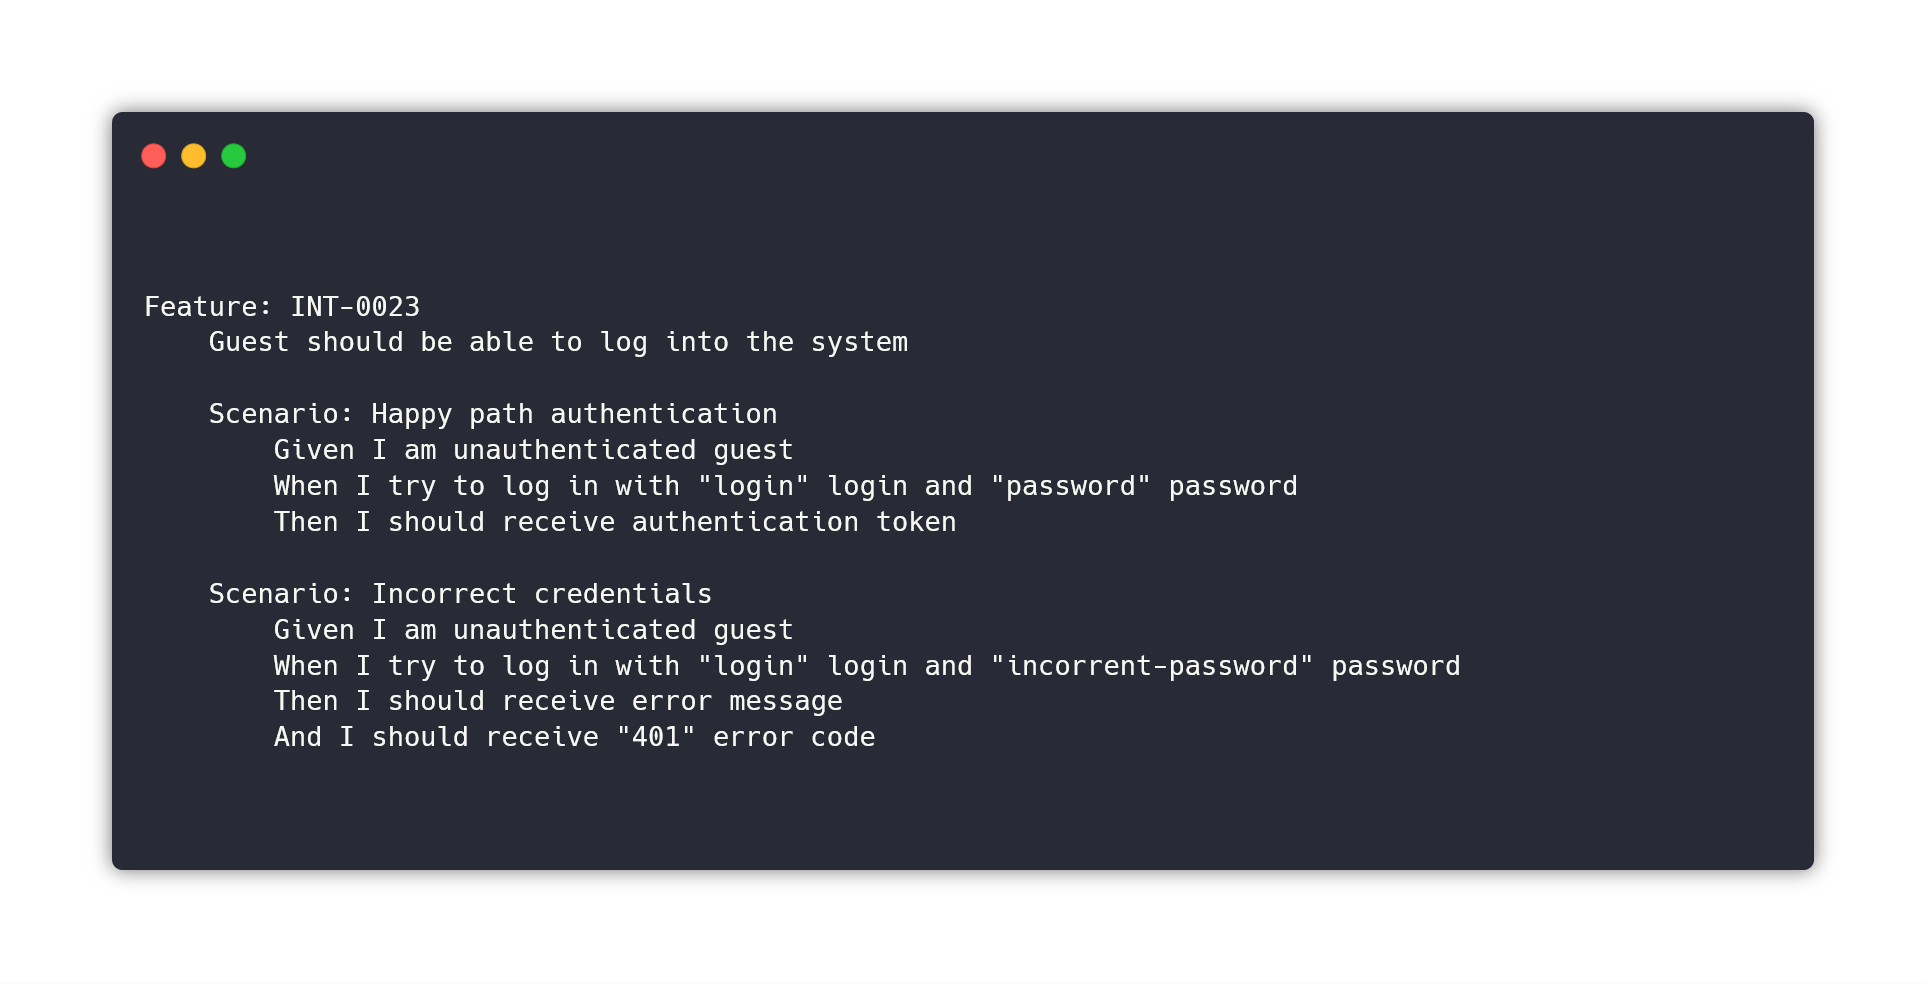
\includegraphics[width=\textwidth]{yagni00.png}
	\end{figure}
\end{frame}

\begin{frame}{YAGNI}
	Co powinniśmy zrobić?
\end{frame}

\begin{frame}{YAGNI}	
	Ustawić routing, przykładowo \texttt{POST /api/login} na kontroler \texttt{AuthenticationController}?
\end{frame}

\begin{frame}{YAGNI}	
	Utworzyć reprezentacje użytkownika dla ORM-a i kontroler?
\end{frame}

\begin{frame}
	\begin{figure} \centering
		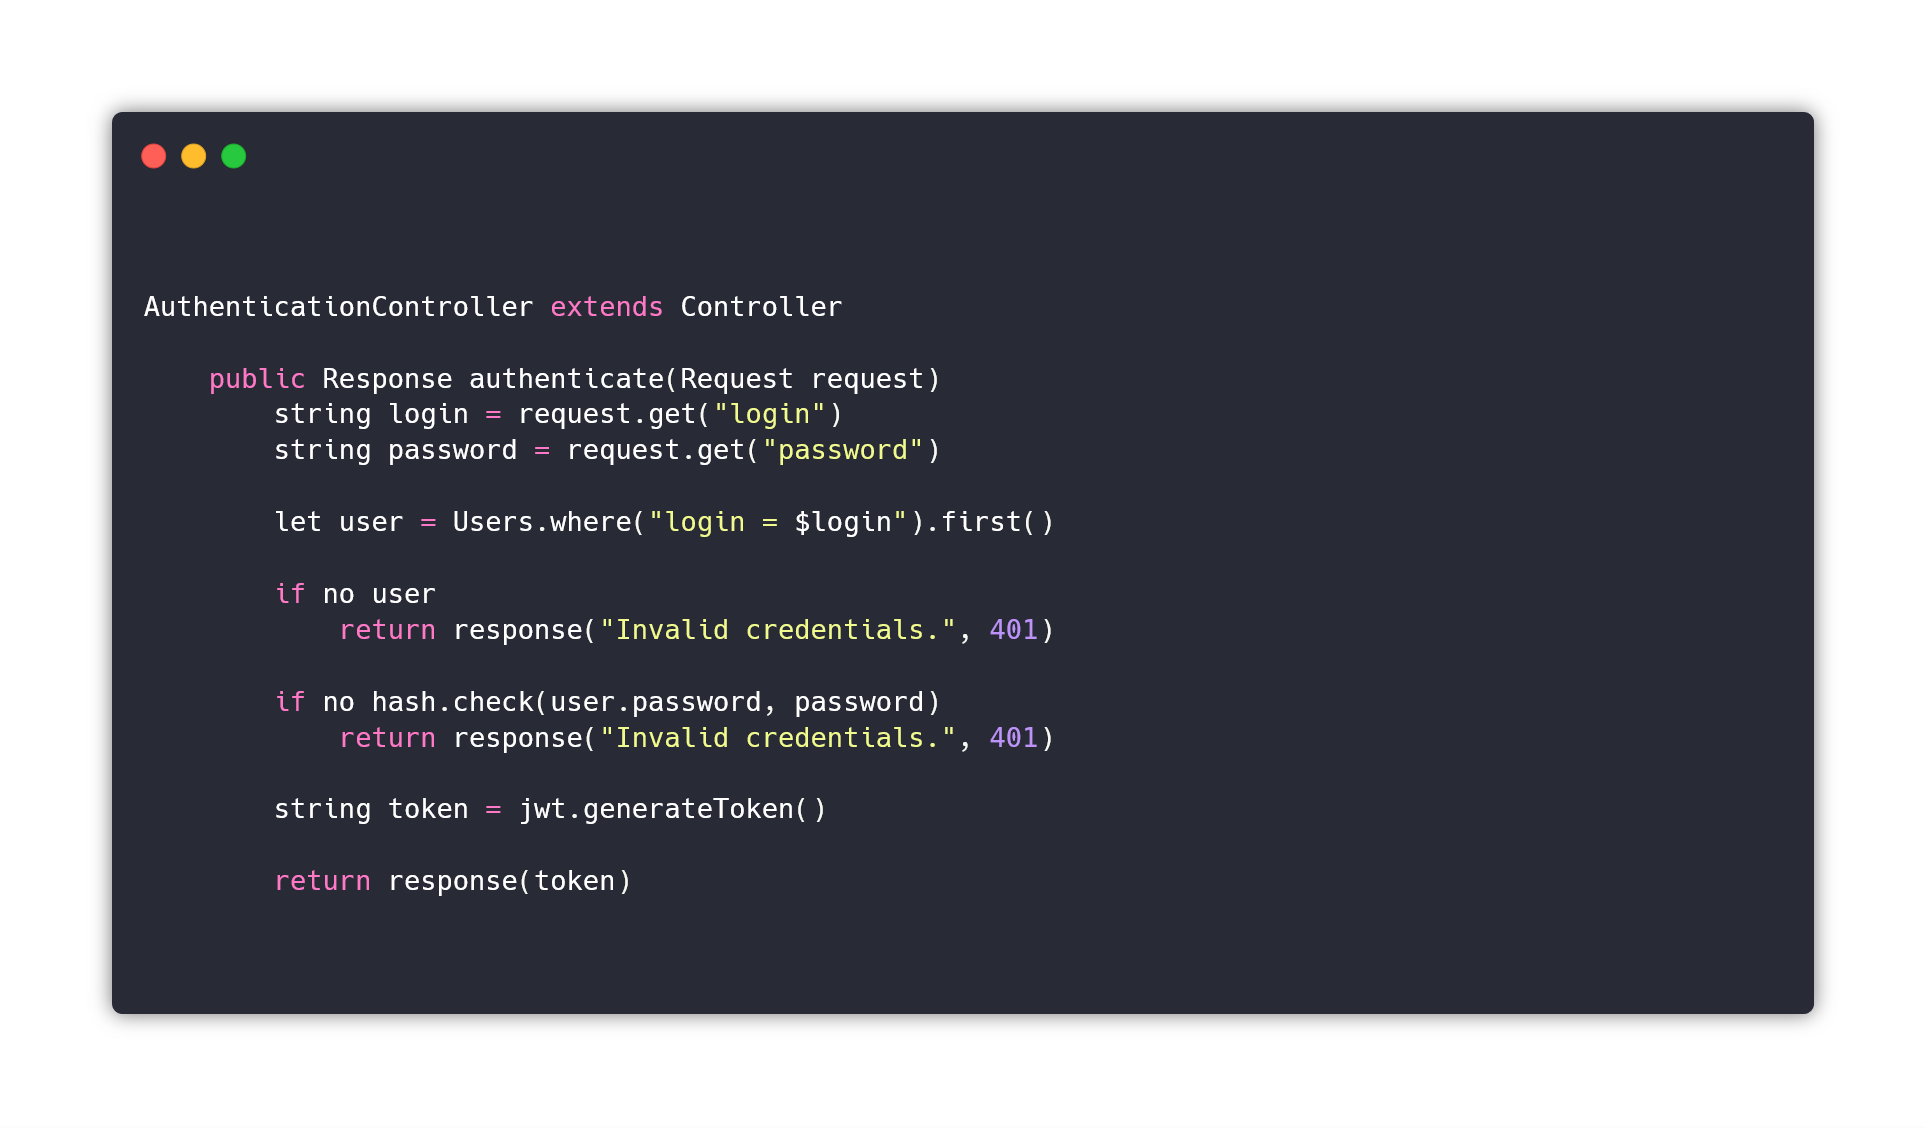
\includegraphics[width=\textwidth]{yagni01.png}
	\end{figure}
\end{frame}

\begin{frame}{YAGNI}	
	Wykonaliśmy zadanie, ale chciałoby się coś jeszcze zrobić, prawda?
\end{frame}

\begin{frame}{YAGNI}	
	Może dodać middleware, które nałożymy na każdy request i sprawdzimy czy mamy przesyłany token? Może wyabstrahować walidację poza kontroler? A może utworzyć dodatkowy serwis do logowania?
\end{frame}

\begin{frame}{YAGNI}		
	No i przecież trzeba zabezpieczyć podanego routa żeby zalogowany użytkownik nie wygenerował sobie nowego tokena. Zróbmy też zwracającą na razie \texttt{true} metodę sprawdzającą czy użytkownik w ogóle może zostać zalogowany; przecież kiedyś wprowadzimy banowanie użytkowników, prawda?
\end{frame}

\begin{frame}{YAGNI}		
	A może w przyszłości będzie więcej niż jeden rodzaj użytkownika, więc wypadałoby nałożyć interfejs na repozytorium użytkowników i wstrzyknąć je do kontrolera? A może przydałoby się opakować token w jakiś uniwersalny view model?
\end{frame}

\begin{frame}{YAGNI}		
	A może w przyszłości będzie więcej niż jeden rodzaj użytkownika, więc wypadałoby nałożyć interfejs na repozytorium użytkowników i wstrzyknąć je do kontrolera? A może przydałoby się opakować token w jakiś uniwersalny view model?
\end{frame}

\begin{frame}
	\begin{figure} \centering
		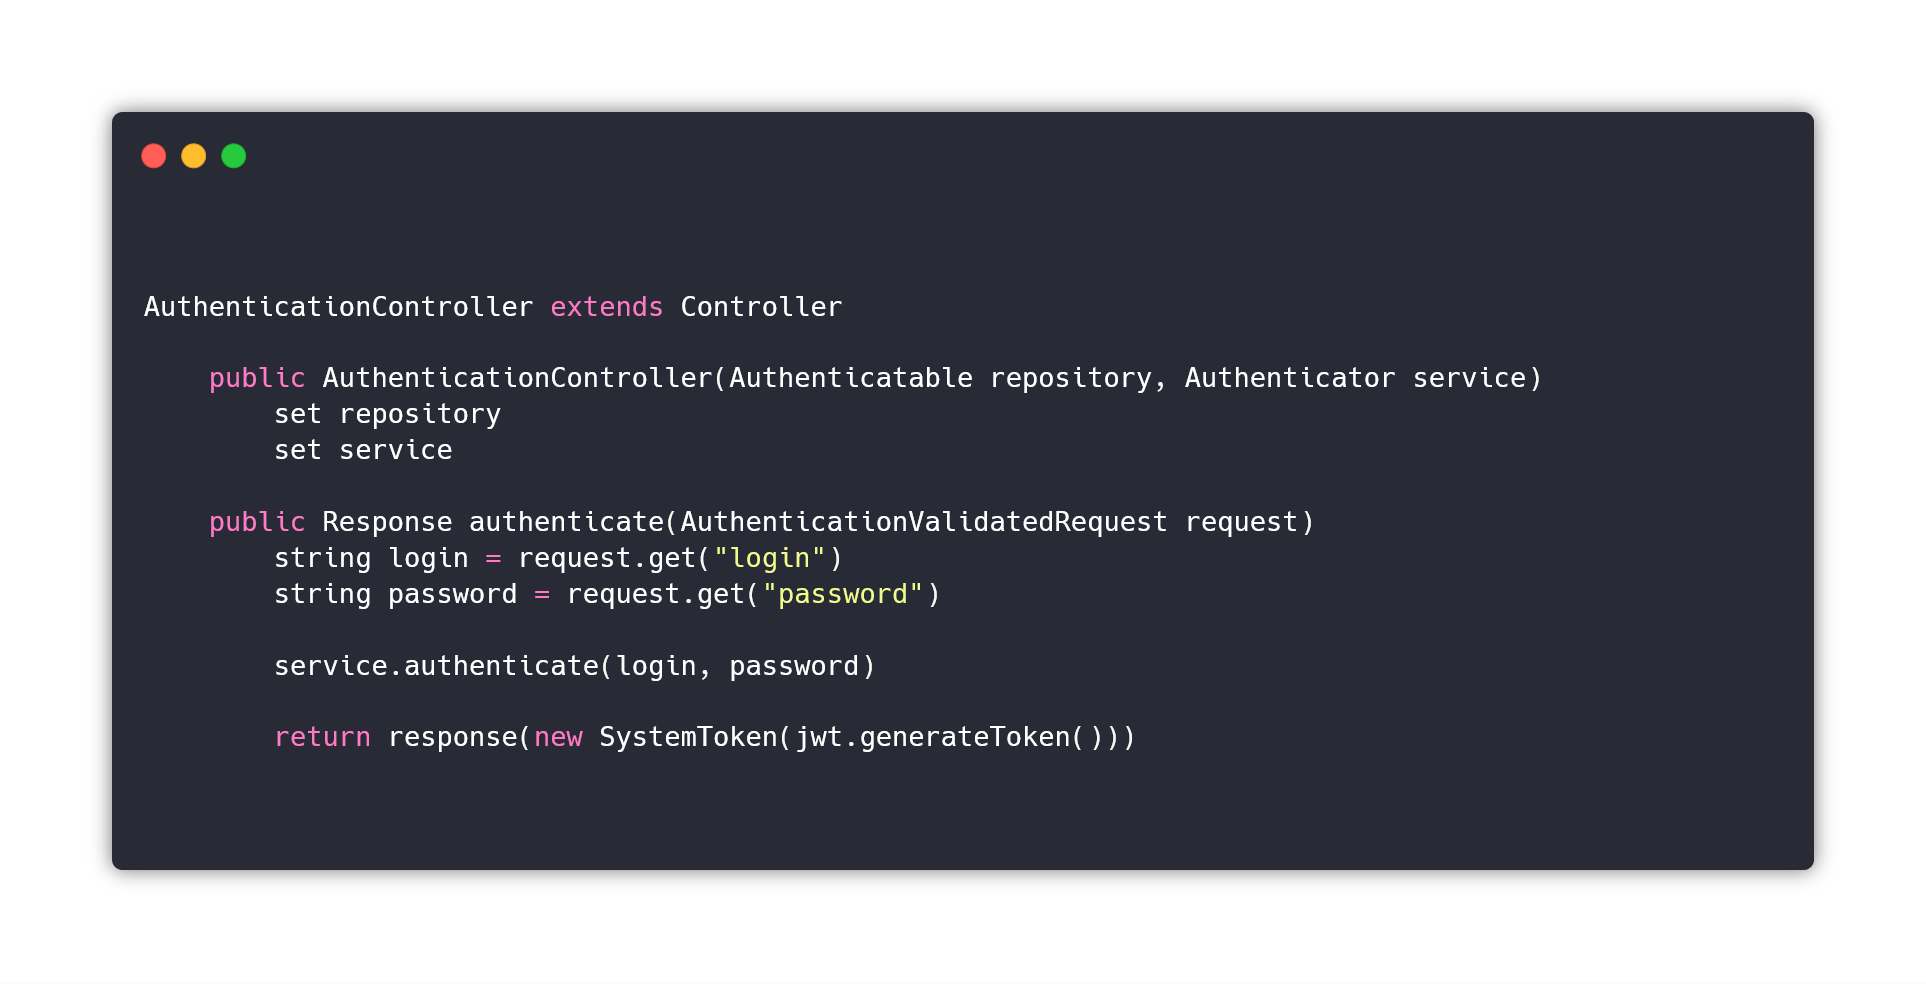
\includegraphics[width=\textwidth]{yagni02.png}
	\end{figure}
\end{frame}

\begin{frame}{YAGNI}		
	Lepiej? Pewnie, że tak! Jest jakby SOLID-niej, jakby czyściej. Kod też się skomplikował, co może być nie do przeskoczenia dla mniej doświadczonych programistów.
\end{frame}

\begin{frame}{YAGNI}		
	Gdzie w tym wszystkim leży YAGNI?
\end{frame}

\begin{frame}{YAGNI}		
	Stety-niestety trzeba wykorzystać własne i cudze doświadczenie oraz zdrowy rozsądek, żeby nakreślić granicę między tym, co warto przewidywać na przyszłość, a tym co powinno pozostać proste.
\end{frame}

\begin{frame}{YAGNI}		
	Na pewno przy takim zadaniu nie powinniśmy jeszcze kombinować z żadnymi middlewarami, żadnymi skomplikowanymi walidacjami, z żadnymi przyszłymi metodami sprawdzania czy ktoś nie został zbanowany.
\end{frame}

\begin{frame}{YAGNI}		
	Dlaczego? Przede wszystkim może to przecież zostać zdefiniowanym w nowych zadaniach, a nie jest w żaden sposób krytyczną funkcjonalnością na obecny moment. Skoro wydzieliliśmy uwierzytelnienie do osobnego serwisu, nie powinno być problemem dodanie później reguł sprawdzających dodatkowe warunki.
\end{frame}

\begin{frame}{YAGNI}		
	Kod powinien być elastyczny, ale na pewno nie rociągnięty. Programistom często się wydaje, że myślą podobnie jak klient. Nigdy nie powinniśmy bez konsultacji dodawać nowych funkcjonalności, bez względu jak \emph{logiczne} mogłoyby się wydawać.
\end{frame}

\begin{frame}{YAGNI}		
	YAGNI nigdy nie powinno być wymówką na tworzenie złego kodu. Powinno byc przestrogą przed tworzeniem niepotrzebnego kodu, który zaciemnia projekt i zwiększa pole do pojawienia się błedów.
\end{frame}

\section{I inne?}

\begin{frame}{I inne}		
	Akronimowych reguł jest wiele, wiele więcej. Czy warto znać wszystkie? Być może.
	
	Ale lepiej po prostu programować, najlepiej w zespole. Wówczas sami dojdziemy do własnych wniosków na temat sensownego wytwarzania oprogramowania.
\end{frame}

\section{Podsumowanie}

\appendix

\begin{frame}[standout]
	Pytania?
\end{frame}

\begin{frame}{}

	Kod prezentacji dostępny jest w repozytorium git pod adresem \texttt{https://bitbucket.org/krewak/pwsz-ppsi} \\ \ \\

	\begin{figure}
		\centering
		\href{https://bitbucket.org/krewak/pwsz-ppsi}{
			
\includegraphics[width=.15\textwidth]{../_template/bitbucket.png}
		}
	\end{figure}
	
	Wszystkie informacje dot. kursu dostępne są pod adresem \texttt{http://pwsz.rewak.pl/kursy/4} \\ \ \\

	\begin{figure}
		\centering
		\href{http://pwsz.rewak.pl/kursy/3}{
			
\includegraphics[width=.15\textwidth]{../_template/rewak.png}
		}
	\end{figure}

\end{frame}

\end{document}
